\chapter{Hierarchical cell type classification using mass, heterogeneous RNA-seq data from human primary cells} \label{chap:2}

The work in this chapter is available as a preprint on bioRxiv (\citealp{Bernstein2019}). 

\section{Background}

Gene expression-based computational classification of a biological sample's constituent cell type is an important task in many gene expression analysis tasks including that of annotating cell types in single-cell RNA-seq datasets (\citealp{Alavi2018, Lin2017}), improving the metadata in public genomic databases (\citealp{Lee2013, Ellis}), and verifying outcomes of experiments that entail inducing cellular differentiation (\citealp{Cahan, Radley2017}).  Furthermore, interpretable cell type classifiers may enable greater understanding of cell-type-specific expression patterns and may prove useful towards efforts, such as the Human Cell Atlas (\citealp{Regev2017}), that seek to define and catalog all cell types in the human body.  The NCBI's Sequence Read Archive (SRA) (\citealp{Leinonen2011}) promises to be a valuable resource for training machine learning algorithms for this task due to the high number and large variety of cell type samples it contains.   However, it has remained underutilized due to both the poor structure of the metadata (\citealp{Goncalves2017}) and the difficulty in obtaining uniformly processed expression data. These challenges have recently been addressed through efficient RNA-seq quantification algorithms (\citealp{Patro2017, Bray2016}) and the metadata normalization efforts discussed in Chapter~\ref{chap:1}, thus paving the way towards the utilization of the SRA for training cell type classifiers. 

In this work, we address three goals pertinent to this task:
\begin{enumerate}
    \item To capture robust cell type signals by training on, and evaluating with, only healthy, primary, purified human samples.
    \item To take advantage of the hierarchical nature of cell type definitions by exploring novel applications of hierarchical machine learning classification methods.
    \item To build interpretable models that can be used to gain deeper understanding into the expression patterns that distinguish cell types.
\end{enumerate}
Existing approaches for cell type prediction address some of these goals, but there has yet to be an investigation that addresses them all simultaneously. 

First, to the best of our knowledge, none of the existing machine learning-based cell type classification approaches that train on public expression data distinguish between treated versus untreated cells (\citealp{Alavi2018, Cahan, Lee2013}). By training on non-primary cells or treated cells, a classifier becomes more susceptible to batch effects when treatment or disease confounds cell type. This also leads to difficulty in model interpretation as it is unclear whether the derived signal is indicative of cell type or of a confounding variable such as treatment or disease. In this work, we compiled a set of training data from the SRA comprising only healthy, primary cells.

We also assert that framing the cell type classification task as that of \textit{multi-label, hierarchical classification} against the Cell Ontology (\citealp{Bard}) poses a number of advantages over flat-classification. The Cell Ontology provides a comprehensive hierarchy of animal cell types encoded as a directed acyclic graph (DAG). This DAG provides a rich source of prior knowledge to the cell type classification task that remains un-utilized in flat classification.

Flat classification suffers from the possibility that predictions are logically inconsistent with the hierarchy of cell types in that the classifier for some cell type may, for a given query, output a probability that is larger than the classifier's output for its parent cell type in the hierarchy (\citealp{Obozinski2008}). Such outputs reduce the interpretability, and therefore scientific usefulness, of the model.  In addition, the use of hierarchical classification approaches allows for the placement of a bulk RNA-seq sample at a level of the hierarchy appropriate to its heterogeneity. For example, a population of cells enriched for T cells may be heterogeneous in the sub-types of T cells (e.g., CD4+ T cells and CD8+ T cells).  

In regards to classification of scRNA-seq data, hierarchical classification allows for informative predictions to be made on query samples whose true phenotype label may not be included in the ontology either because the ontology is incomplete or that phenotype has yet to be discovered. Finally, by utilizing the hierarchy during training rather than using flat classification, more accurate classifiers can be learned (\citealp{BarutcuogluSchapireTroyanskaya2006}). 

To the best of our knowledge, only work by  \cite{Kanter2019} and \cite{Lee2013} frames the cell type prediction task as a hierarchical classification problem.  \cite{Kanter2019} developed an algorithm called CHETAH that learns a hierarchy from the training data; however, this algorithm does not take advantage of the rich hierarchy of cell types already available in biomedical ontologies.  \cite{Lee2013} developed an algorithm called URSA that does utilize a pre-existing ontology of tissues and cell types, and to this end, train a hierarchical classifier using Bayesian Network Correction (BNC) (\citealp{BarutcuogluSchapireTroyanskaya2006}). However, there also exist discriminative methods for hierarchical classification that have yet to be applied to the cell type prediction task. Thus, we applied a number of such approaches including cascaded logistic regression (CLR), isotonic regression correction (IR) (\citealp{Obozinski2008}), and a heuristic procedure called the True Path Rule (TPR) (\citealp{Notaro2017}). We compared these discriminative methods to BNC and in our hands found them to outperform the BNC approach.

Furthermore, we sought for our methods to be interpretable in order for our trained classifiers to be of use not only in classification, but also for investigating cell type-specific expression patterns. To this end, this work makes extensive use of linear models, which are particularly amenable to interpretation. We tested the interpretability of the aforementioned frameworks and found that CLR is particularly interpretable as it is able to delineate functional differences between similar cell types.

We tested these algorithms on single-cell RNA-seq (scRNA-seq) data, resulting in promising performance. We propose that hierarchical, machine learning-based classification of single-cell expression data will help overcome a number of challenges in cell type labeling of single-cell datasets.  Currently, labeling cell types in scRNA-seq data is an ad hoc process that involves clustering the cells and then searching for differential expression of certain cell-type-specific marker genes across these clusters. This process is challenged both by the fact that there is not a canonical set of marker genes for most cell types (\citealp{Zhang2018}) and that this process is affected by the clustering algorithm (\citealp{Kiselev2019}). Approaches are beginning to emerge that rely on training cell type classifiers on single-cell data (\citealp{Xie2019, Alavi2018}).  

We note that the process of training a cell type classifier on single-cell data is somewhat circular in that the ground truth cell type labels are most commonly based upon gene expression (via the expression of cell type-specific marker genes), which is then also used for constructing the machine learning features.  In this work, we train our algorithms on only bulk RNA-seq data, that originate from cells that have been isolated based on phenotypic characteristics downstream of gene expression itself (such as cell surface proteins). Thus, we suggest that bulk RNA-seq data in the SRA cannot only be utilized, but also may be preferred, for the training of cell type classifiers applied towards scRNA-seq datasets. 

Finally, we created a Python package, CellO (\textit{Cell} \textit{O}ntology-based classification) that allows users to run pre-trained classifiers on their own RNA-seq data. CellO is available at \ClassifierURL{}.

\section{Results and discussion}

\subsection*{A novel curated RNA-seq dataset of human primary cells}\label{sec:primary_cell_data}

In order to capture robust cell type signals, we sought a dataset of RNA-seq samples comprising only healthy primary cells. We did not wish to include cells that underwent multiple passages, were diseased, or underwent other treatments, such as in vitro differentiation, because these conditions alter gene expression. We therefore curated a novel dataset from the SRA consisting of healthy, untreated, primary cells.  We leveraged the annotations provided by the MetaSRA, which includes sample-specific information including disease-state, treatment, and sample type (i.e., their status as primary cells). Consequently, we followed the conservative definition for a primary cell sample according to the criteria laid out in Chapter~\ref{chap:1}, which requires that a sample has not undergone passaging beyond the first culture.  We used the MetaSRA to capture an initial candidate set of primary samples and then within this set, manually annotated these samples for technical variables (such as bulk vs. single-cell status) by consulting sources of metadata that are not captured by the MetaSRA annotation process such as fields in Gene Expression Omnibus (\citealp{Barrett2013}) records and each study's publication.  When found, we corrected errors in the MetaSRA-provided Cell Ontology labels. 

This process resulted in a dataset comprising \TotalExperiments{} total samples.  We uniformly quantified and normalized (via log counts per million) gene expression from the raw RNA-seq data for these samples.  Of these samples, \ExperimentsInBulkDataset{} were bulk RNA-seq samples from \StudiesInBulkDataset{} studies and labeled with \CellTypesInBulkDataset{} cell type terms in the Cell Ontology. Of these cell types, \MostSpecificBulkCellTypes{} cell types were the most-specific cell types in our dataset (i.e., no sample in our data was labelled with a descendent cell type term). These cell types were diverse, spanning multiple stages of development and differentiation (Fig.~\ref{fig:dataset_summary}). To the best of our knowledge, this dataset is the largest and most diverse set of bulk RNA-seq samples derived from only primary cells.  Prior to this work, the most comprehensive bulk primary cell transcriptomic dataset was compiled by Aran \textit{et al.} (2017), which contained data for 64 cell types from 6 studies.  Whereas our dataset consists of only RNA-seq data, this prior dataset included samples assayed with several other technologies, such a microarrays.  In addition to bulk samples, our dataset also includes \ExperimentsInSingleCellDataset{}  single-cell samples from \StudiesInSingleCellDataset{} studies and labeled with \CellTypesInSingleCellDataset{} cell types. We note that this data includes single-cell samples from protocols such as MARS-seq (\citealp{Jaitin2014}) and SMART-Seq2 (\citealp{Picelli2013}), but it does not include data from droplet-based protocols such as Chromium 10x. Chapter~\ref{chap:3} will address cell type prediction on RNA-seq generated from these more novel technologies.


\clearpage
 \begin{sidewaysfigure}
    \thispagestyle{empty}
    %\vspace{-4.5cm}
    \centerline{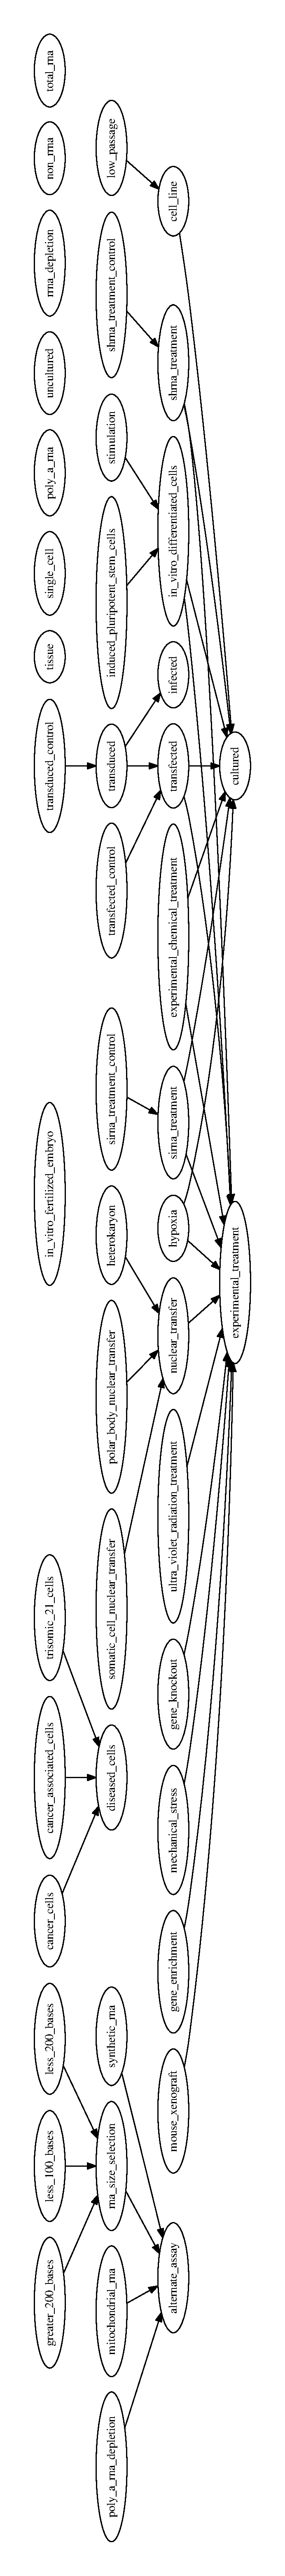
\includegraphics[scale=0.24, angle=-90]
    {figures/tags.pdf}}
    \caption{\textbf{Custom technical label graph.} We created a custom hierarchy of technical variables, in the form of a directed acyclic graph, in order to annotate the technical variables in the retrieved RNA-seq samples. Edges in the graph indicate an ``is a" relationship between terms.  We partitioned and filtered the candidate set of primary cell samples based on their labels within this technical variables hierarchy.  For example, we created separate bulk and single-cell RNA-seq datasets. In addition, we used this hierarchy to exclude any samples for which the RNA underwent size-selection, that were associated with disease, or treated.  We did, however, choose to include those samples that were treated with a ``control" treatment (e.g., labelled with ``transformed\_control").  Our inclusion criteria removed any samples that underwent multiple passages in culture or were induced into in vitro differentiation or activation.}
    \label{fig:tech_labels}
      \end{sidewaysfigure} 

  \begin{figure}[h!]
    \centerline{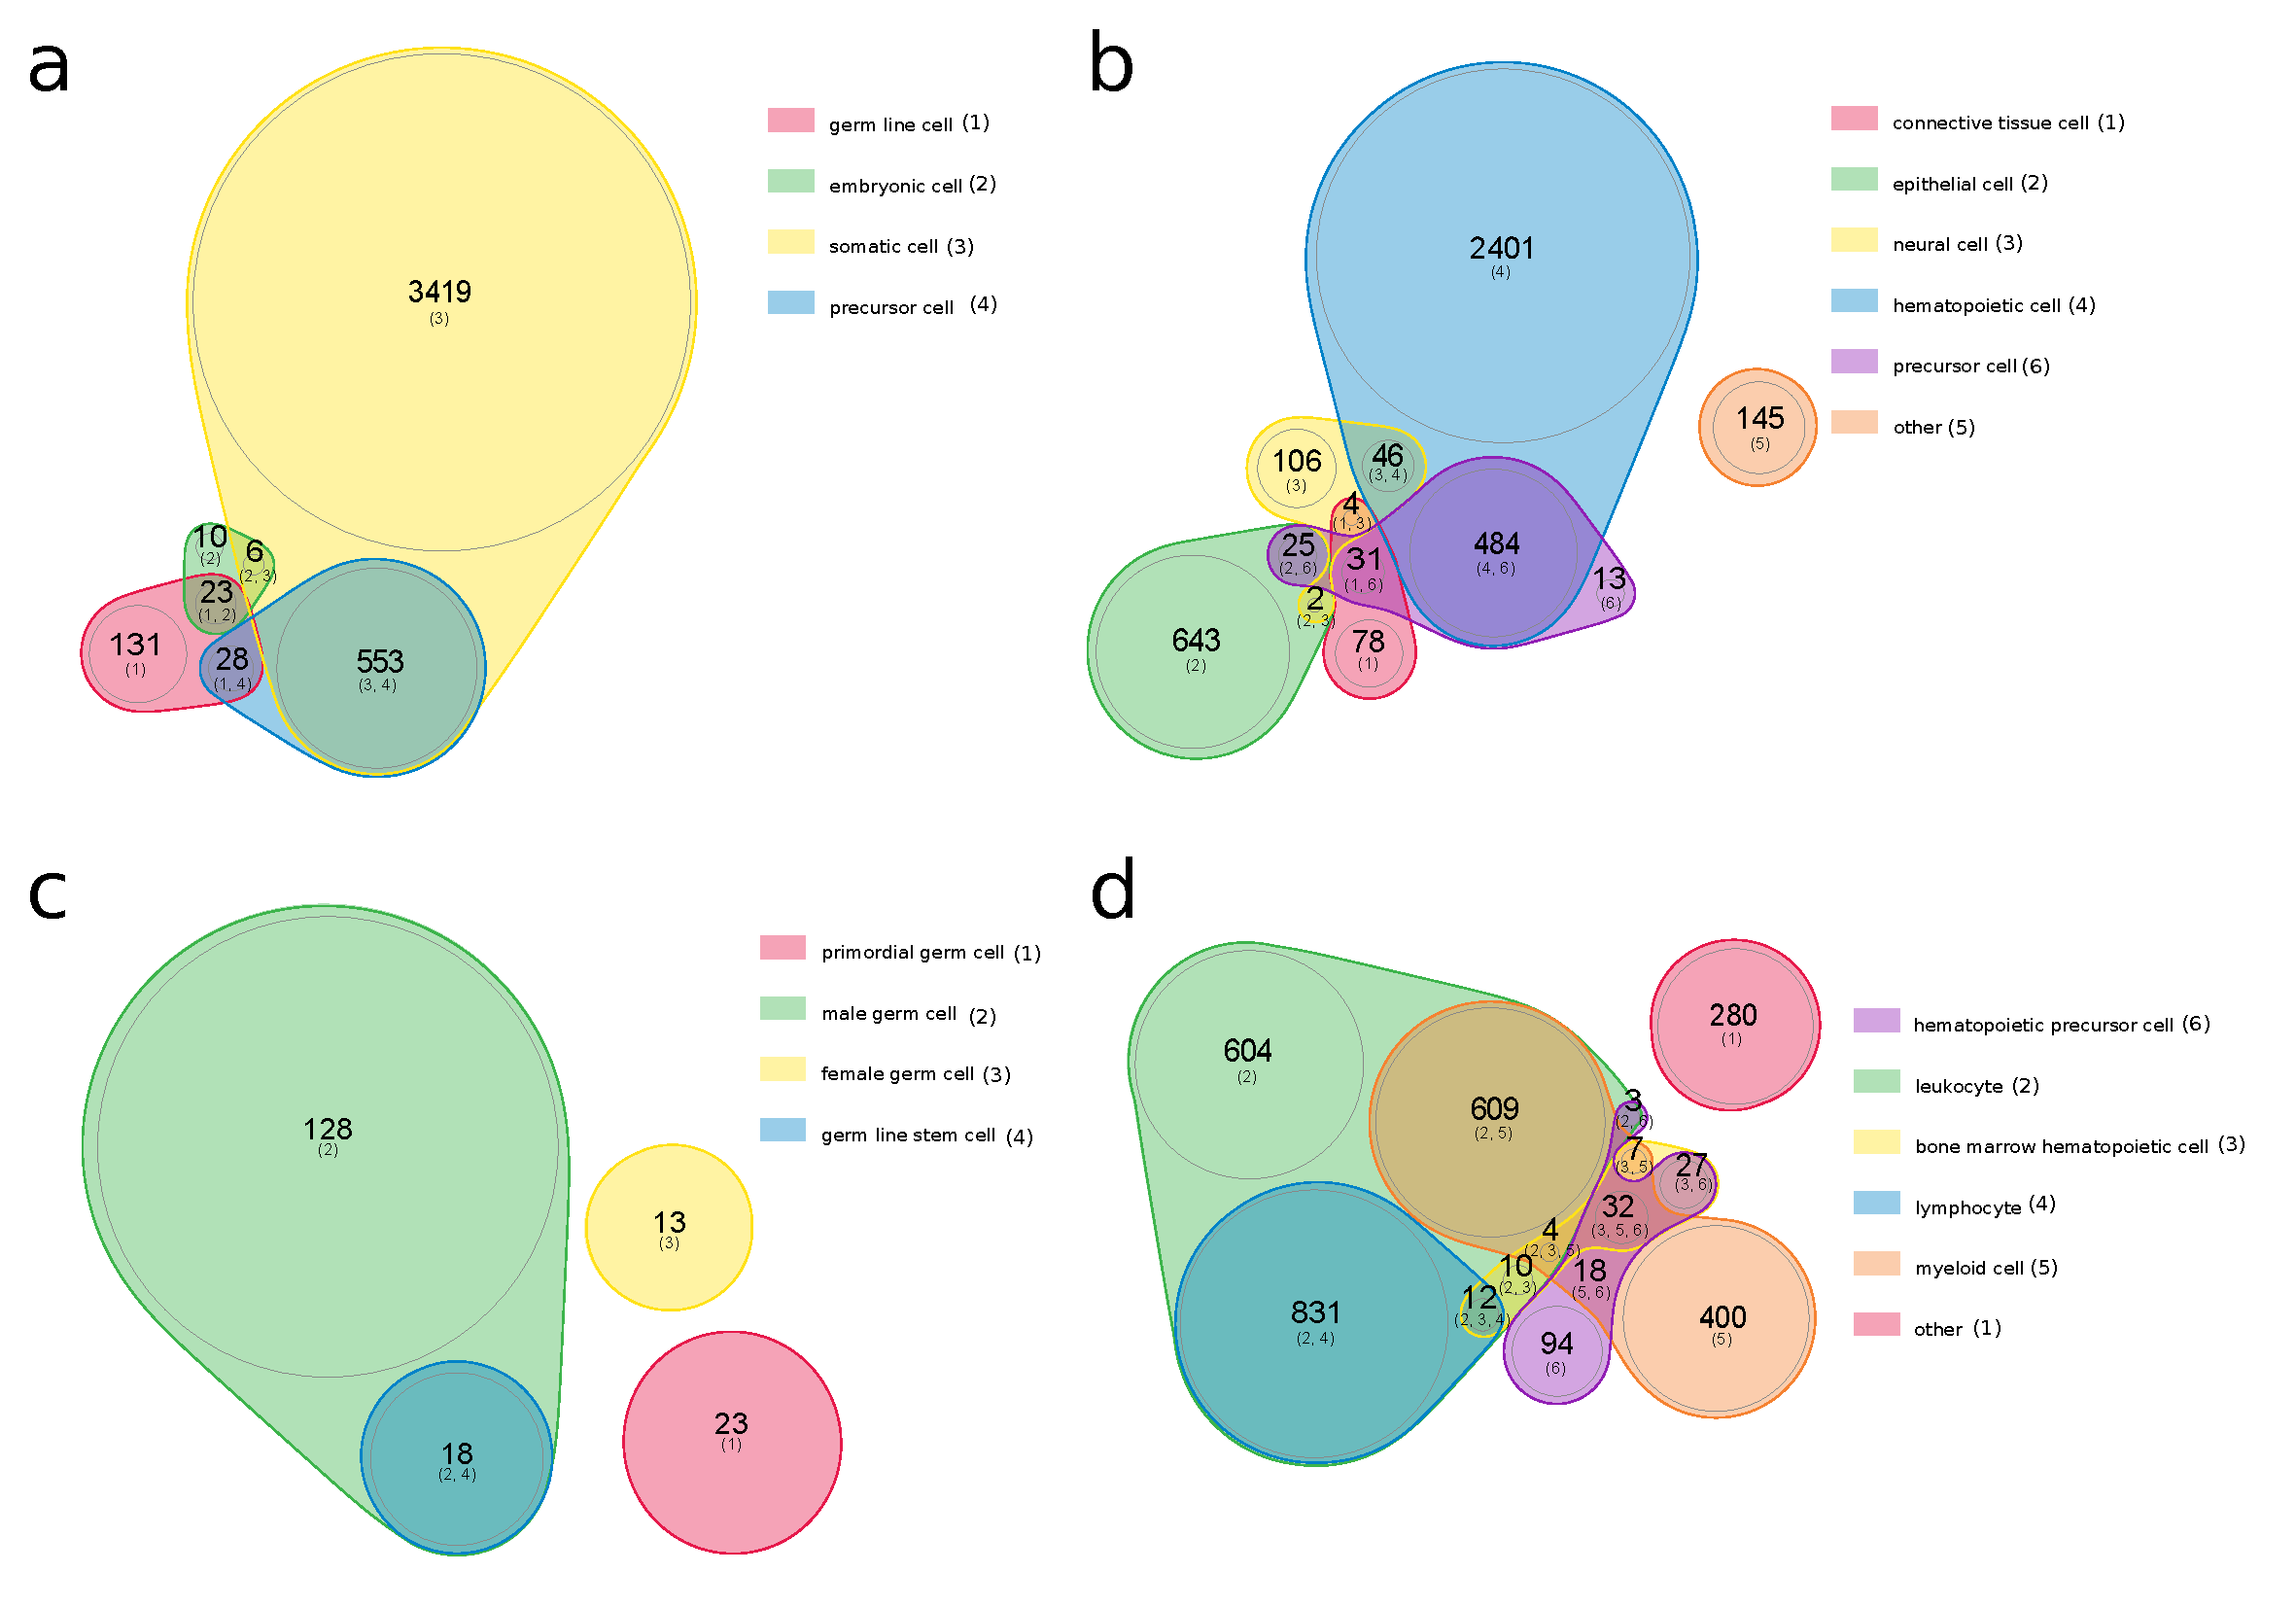
\includegraphics[width=13cm]{figures/data_venn.pdf}}
    \caption{
      \textbf{Primary cell dataset summary.} Euler diagrams of the cell types in the bulk RNA-seq data set divided by (\textbf{a}) broad cell types, (\textbf{b}) somatic cell types, (\textbf{c}) germ line cell types, and  (\textbf{d}) hematopoietic cell types. Diagrams were created with nVenn (\citealp{PerezSilva2018}). }
    \label{fig:dataset_summary}
      \end{figure}

To evaluate the implemented machine learning methods on their ability to classify bulk RNA-seq data, we split the bulk RNA-seq data set into a training and a test set, ensuring both that samples from the same study were never split across the training and test sets and that the training and test partitions had a high overlap of cell types. This partition yielded a training set with \ExperimentsInBulkTrainingDataset{} samples across \StudiesInBulkTrainingDataset{} studies and a test set with \ExperimentsInBulkTestDataset{} samples across \StudiesInBulkTestDataset{} studies. The training set and test set shared \NumCellTypesIntersectTrainingTest{} cell types. 

We separately evaluated these methods on their ability to classify scRNA-seq data. To this end, we created a second test set of all single-cell samples whose cell types appeared in the bulk RNA-seq data. This resulted in a test set of \BulkRestrictedSingleCellExperiments{} samples across \BulkRestrictedSingleCellStudies{} studies from \BulkRestrictedSingleCellCellTypes{} cell types. As detailed below, we separately examined how the classifiers handled the remaining single-cell samples whose cell types do not appear in the bulk RNA-seq training data.

\subsection*{Novel applications of hierarchical classification methods}

One straightforward approach to performing cell type prediction against the Cell Ontology entails training an independent binary classifier for each cell type in the ontology.  We will refer to this as the ``independent classifiers'' approach.  Such an approach suffers from the possibility that the classifiers' outputs will be inconsistent with the hierarchical structure of the ontology. An inconsistency occurs when the output probability for a given cell type exceeds that of one of its parent cell types in the ontology. We tested the use of independent classifiers and found inconsistencies to be an important source of errors. Specifically, we trained independent, one-vs.rest cell type classifiers on the bulk RNA-seq training set, applied them to the test set, and then examined the consistency of all edges that were adjacent to at least one cell type whose classifier produced a non-negligible probability ($> 0.1$) of the sample originating from that cell type (Fig.~\ref{fig:cdf_incons}).  Of these edges, \FracEdgesInconsistent{} were inconsistent.

\begin{figure}[htbp]
    \centerline{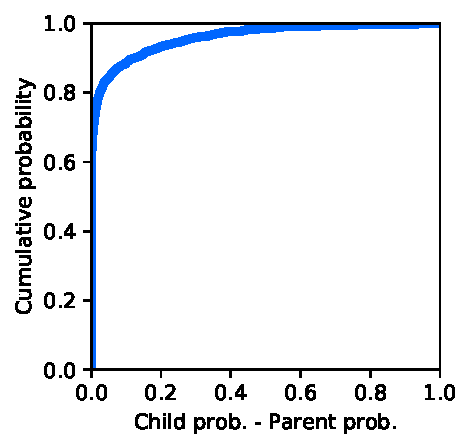
\includegraphics[scale=1.0]{figures/CDF_inconsistences.pdf}}
    \caption{\textbf{Distribution of edge inconsistencies.} The cumulative distribution function over the difference in probability between the parent and child classifiers for all edges for which either the parent or child classifier output a probability greater than 0.01.  A total of \EdgesSeverelyInconsistent{} edges saw a difference in probability greater than 0.5 which constitutes approximately one severely inconsistent edge for every ten samples.}
    \label{fig:cdf_incons}
      \end{figure} 

Hierarchical classification algorithms ensure that the output probabilities are consistent with the ontology. We tested three ensemble-based hierarchical classification algorithms that have yet to be applied to the gene expression-based cell type prediction task: cascaded logistic regression (CLR), isotonic regression correction (IR) (\citealp{Obozinski2008}), and a heuristic procedure called the True Path Rule (TPR) (\citealp{Notaro2017}). Cascaded logistic regression entails classifying a sample in a top-down fashion from the root of the ontology downward via an ensemble of binary classifiers. Specifically, each binary classifier is associated with a cell type and is trained to classify a sample conditioned on the sample belonging to all of the cell type's parents in the ontology. In contrast, IR and TPR train independent, unconditional, one-versus-rest binary classifiers for each cell type and then, for a given query sample, reconcile the output of these independent classifiers to be consistent with the ontology. IR uses a projection-based approach for reconciliation, that entails finding a set of consistent output cell type probabilities that minimize the sum of squared differences to the raw, and possibly inconsistent, classifier output probabilities. In contrast, TPR uses a heuristic procedure that involves a bottom-up pass through the ontology such that the output of children classifiers are averaged with the output of the parent classifier to allow information flow across the ontology graph.

To date, the one hierarchical classification method that has been applied to the task at hand is BNC (\citealp{BarutcuogluSchapireTroyanskaya2006}), and therefore, as a baseline, we implemented a BNC algorithm following the description in \cite{Lee2013}.  We tested a number of variants of this algorithm and report here the best-performing variant (Fig.~\ref{fig:bncvariants}).  Lastly, as a na\"ive baseline, we implemented a one-nearest-neighbor algorithm that simply returns the cell type labels of the most similar sample in the training set to the query sample using Pearson correlation as the similarity metric.  

\begin{figure}[htbp]
    \centerline{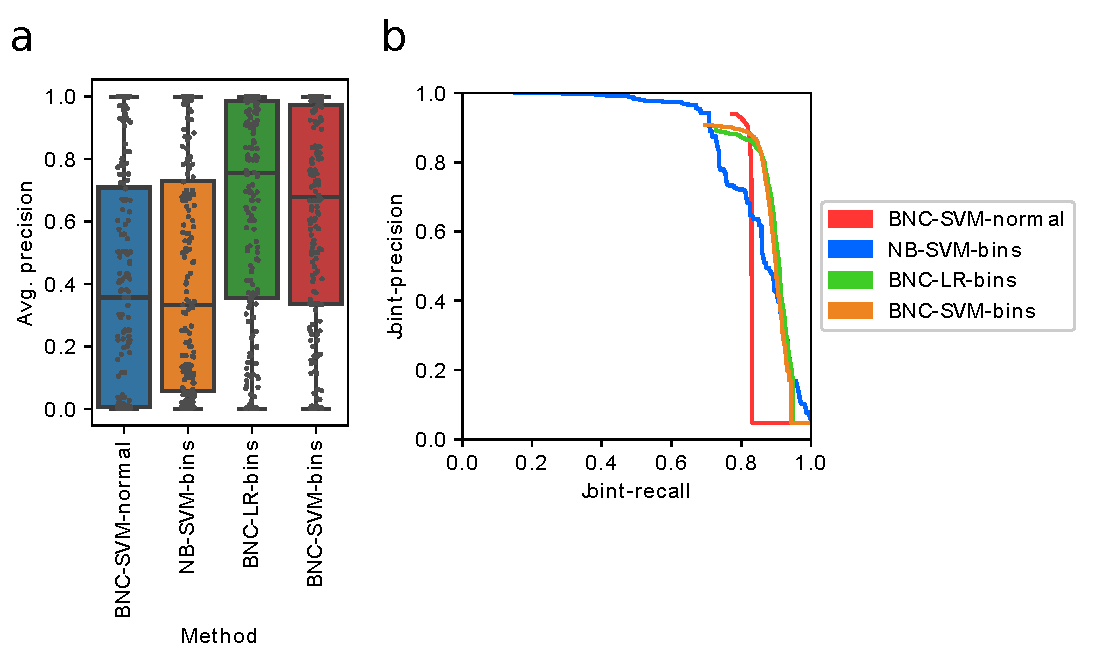
\includegraphics[width=13cm]{figures/bulk_test_bnc_results.pdf}}
    \caption{\textbf{Performance of BNC variants.} Analysis of four variants of the BNC algorithm on the bulk RNA-seq test set.  We compared a variant that uses normal distributions instead of bins (BNC-SVM-normal), a naive Bayes algorithm (NB-SVM-bins), and a variant that uses logistic regression instead of SVMs (BNC-LR-bins) to the approach used in the paper (BNC-SVM-bins). We compared these methods using the per-cell type mode of evaluation in which we compare the distributions of cell type average precision scores (a) as well as the joint mode of evaluation in which we compare the joint precision-recall curves (b).}
    \label{fig:bncvariants}
      \end{figure}

We performed three modes of evaluation: per-cell-type, per-sample, and joint (\citealp{Obozinski2008}). In the per cell type mode of evaluation we evaluate the performance of each method on each cell type independently. The results of this mode of evaluation are provided for users who are interested in examining each method's performance on specific cell types. Specifically, for each cell type, we compute both the average precision (a measure of the area under the precision-recall curve) as well as the maximum achievable recall at 0.9 precision. This latter metric is provided for users who cannot tolerate low precision. 

In the per-sample mode of evaluation, we examine the average performance of the classifiers on a per-sample basis.  To this end, we used two variants of precision and recall that are sample-centric. Given a sample, the first variants are the standard precision and recall over the sample's true cell types and predicted cell types. The second variants, which we call \textit{specific-precision} and \textit{specific-recall}, take into account only the sample's most-specific true cell types and predicted cell types according to the ontology (i.e., the deepest terms in the ontology -- see Methods).  Then, for a given prediction threshold, we compute the mean precision and recall (as well as mean specific-precision and mean specific-recall) across all samples. By varying our prediction threshold, we compute a \textit{mean precision-recall curve}, where an operating point on this curve describes an achievable mean precision and mean recall across all samples. 

A disadvantage to these mean precision and mean recall metrics is that they can be dominated by large studies due to samples from the same study sharing batch effects and similar cell type labels. To counteract this, we also compute curves in which in our calculation of the mean precision and mean recall at a given threshold down-weights samples according to the number of samples in its study in order to ensure that each study contributes equally to the mean precision-recall curve. We refer to these curves as \textit{study-weighted, precision-recall curves}. An operating point on such a curve describes an expected precision and recall that is achievable given that a study is first sampled uniformly from all available studies, and then an RNA-seq sample is sampled uniformly from that study. 

Lastly, for each method, we performed a joint evaluation that entailed treating each paired sample and cell type prediction independently. The set of all such predictions was ordered according to prediction probability and the corresponding precision-recall curve was constructed.

\subsection*{Advantages of training on data from heterogeneous sources}

We hypothesized that by leveraging data from multiple studies, we could mitigate the models fitting a single study's batch effects, and would therefore learn more robust signals for each cell type.  We tested this hypothesis using a flat classification experimental setup in which the hierarchy of cell types was first ignored.  Specifically, for a variety of cell types, we compared the performance between logistic regression binary classifiers trained on homogeneous data (data originating from a single study) versus those trained on heterogeneous data (data originating from different studies). 

The experiment proceeded as follows: we first queried the bulk RNA-seq data for all cell types that included at least three studies with over 10 experiments for that cell type. For each of these cell types, $c$, we partitioned the data labelled with $c$ according to their study of origin, and then iteratively held out each study-partition as a test set. From the remaining held-in partitions, we constructed two sets of training sets. The first set of training sets included positive examples (i.e. data labeled with $c$) from only one study, which we call \textit{homogeneous training sets}. The second set of training sets included positive examples from all held-in study-partitions, which we call the \textit{heterogeneous training sets}. For all training sets, we use a consistent set of negative examples randomly chosen from the samples that are not labelled as $c$.  Furthermore, when constructing each training set, we ensured each had an equal number of positive examples. We then trained a binary classifier on each training set and evaluated them on the held-out study-partition. Figure~\ref{fig:homo_vs_hetero_setup}a provides a schematic of the experiment (See Supplementary Materials for full details).  We computed the mean average-precision for the homogeneously trained and heterogeneously trained classifiers across each held out study-partition and cell type pair and  found that heterogeneously trained classifiers tended to have a higher mean average precision (Fig.~\ref{fig:homo_vs_hetero_setup}b).  These results support the hypothesis that better generalization can be achieved by training on data from multiple studies.

  \begin{figure}[h!]
  \centerline{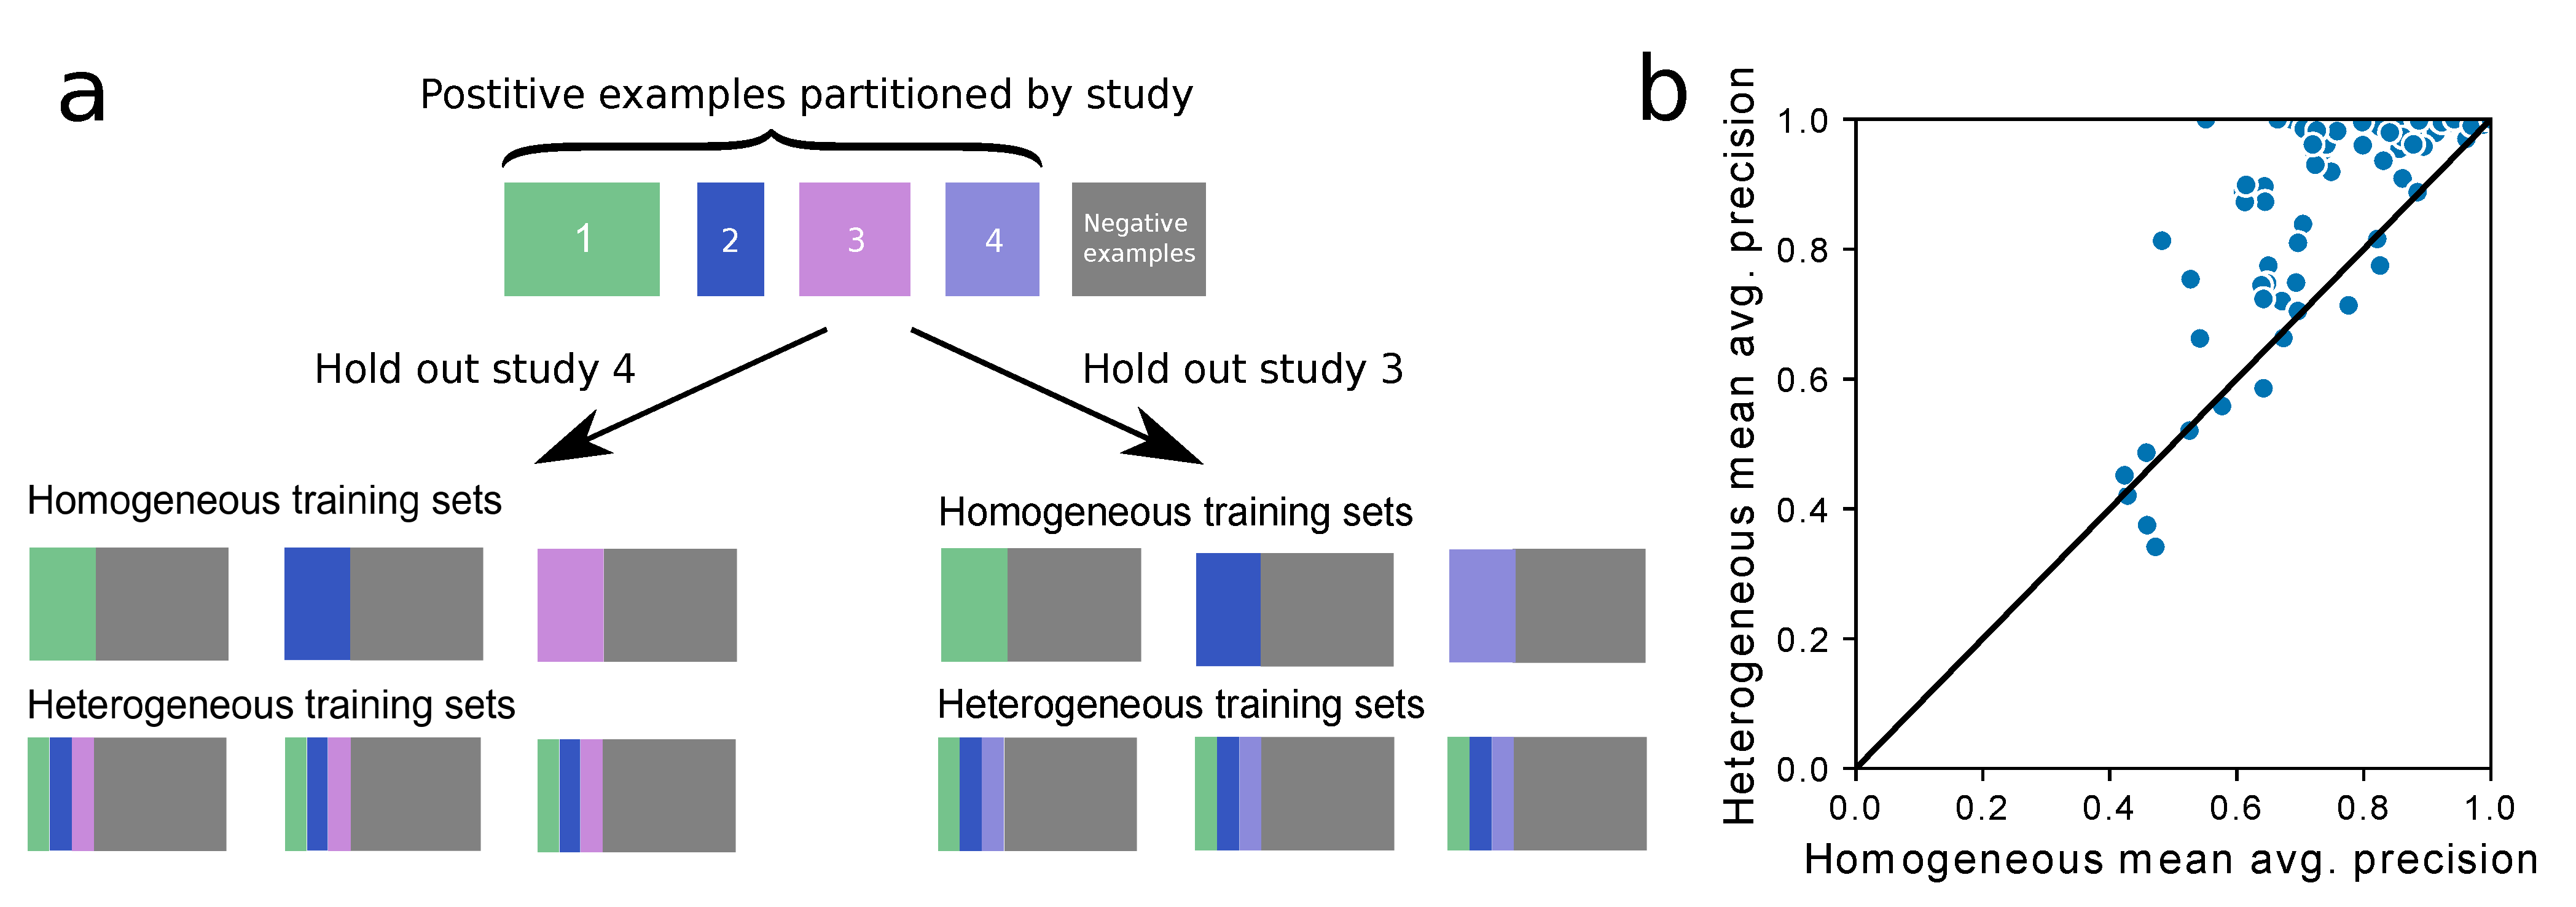
\includegraphics[width=13cm]{figures/homo_vs_hetero_full.pdf}}
  \caption{
     \textbf{Examining the effects of training on heterogeneous data.} (a) A schematic illustrating the experimental setup for our investigation into the effects of training on data from multiple studies versus training on data from a single study.  For a given cell type, we find all studies that contained at least ten samples for that cell type. The numbered colored rectangles illustrate such samples partitioned by their study. We then hold out each study and construct two sets of training sets -- one set of homogeneous training sets and another of heterogeneous training sets.  A classifier is trained on each training set and evaluated on data in the held out study. Above, we illustrate the training sets constructed when holding out studies 3 and 4. Each training set uses an identical set of negative examples and identical sized sets of positive examples (the minimum number of samples in a given study partition). (b) Comparing the mean-average precision across cell types between the homogeneously trained classifiers and the heterogeneously trained classifiers on each held out study.}
      \label{fig:homo_vs_hetero_setup}
      \end{figure}


\subsection*{Evaluation on bulk RNA-seq data}

We evaluated the aforementioned hierarchical classification algorithms using the per-cell type (Fig.~\ref{fig:results_test_bulk}a-b, Fig.~\ref{fig:bulk_pairwise}), per-sample (Fig.~\ref{fig:results_test_bulk}c), and joint (Fig.~\ref{fig:results_test_bulk}d) modes of evaluation.  Overall, we find that IR, TPR, CLR, and independent classifiers performed similarly and better than the baseline BNC and nearest-neighbor algorithms. The similar performance of IR, TPR, and CLR to the independent classifiers demonstrates that reconciling the outputs of the independent predictions with the ontology structure does not degrade performance.  We note that these results are in line with work by Obozinski \textit{et al.} (2008), which demonstrates that IR and CLR outperform BNC on the hierarchical protein function prediction task.

Regarding the per-sample mode evaluation, we note that mean performance on a sample's most-specific cell types was below that of the mean performance when considering all of the sample's cell types (Fig.~\ref{fig:results_test_bulk}c).  We posit three reasons for this: first, it is likely easier for the classifiers to distinguish broad categories of cell types than it is to distinguish fine-grained cell types for which cell-type-specific expression signatures may be more subtle. Second, the amount of training data supporting each cell type strictly decreases down the ontology. Third, we note that a subset of the errors are due to the classifiers providing significant probability to more specific cell types than the most-specific true cell types for a given sample (e.g., a T cell sample predicted to be a CD4+ T cell sample). This may be due to the prevalence of an unlabeled, more-specific cell type in some heterogeneous bulk RNA-seq samples.     

\begin{figure}[h!]
      \centerline{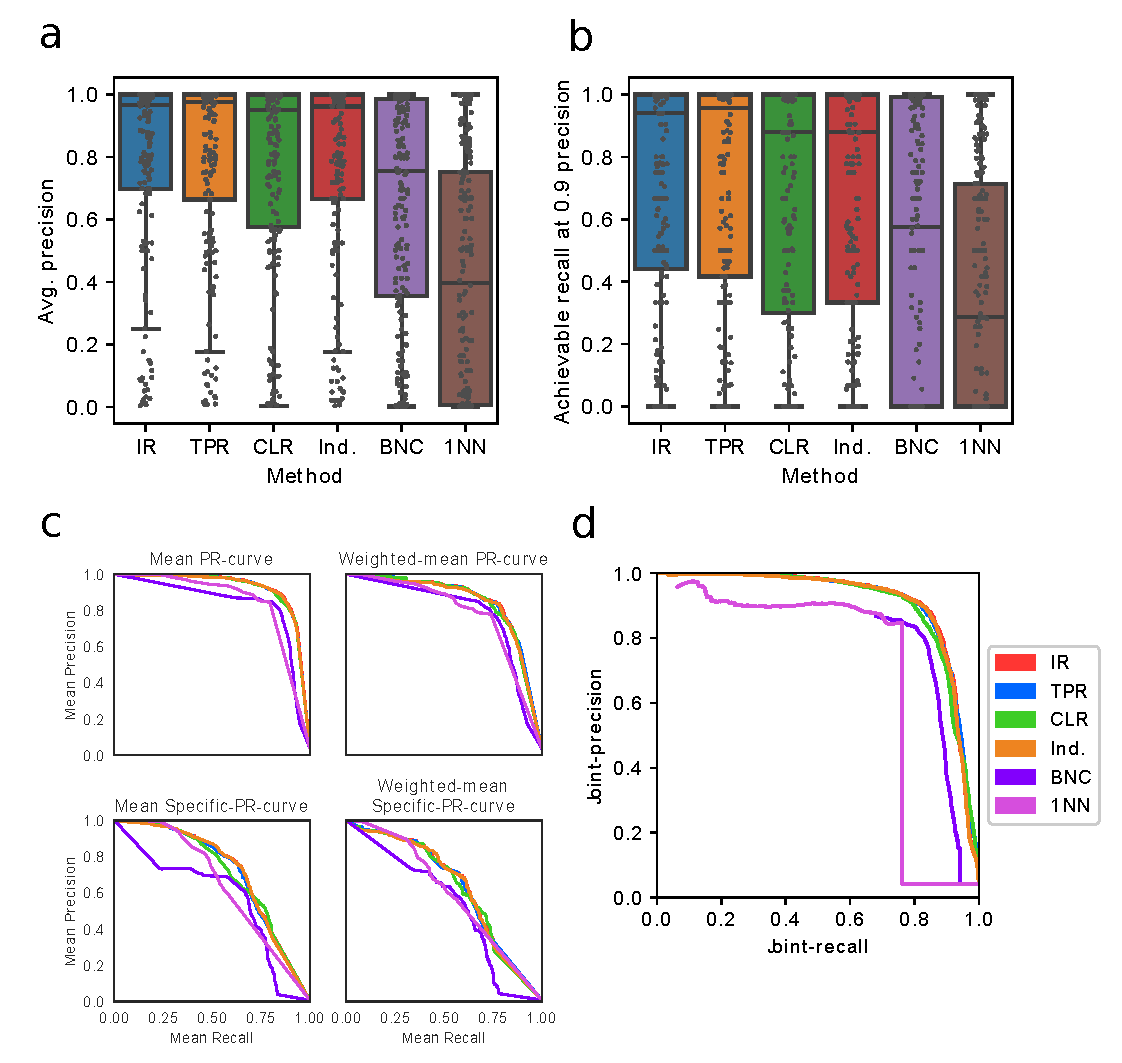
\includegraphics[width=13cm]{figures/bulk_test_set_results.pdf}}
      \caption{\textbf{Bulk test set results.} (a) Comparison between the distributions of average-precision generated by each method across all cell types.  (b) Comparison of the distributions over the highest achievable recalls when precision is fixed at 0.9 across all cell types. (c) Variants of the mean precision-recall curves for comparing the average performance of each method across all samples. (d) The joint-precision recall curves for all methods generated by ranking all sample-cell type output probabilities jointly.}
      \label{fig:results_test_bulk}
      \end{figure}

\begin{figure}[htbp]
    \centerline{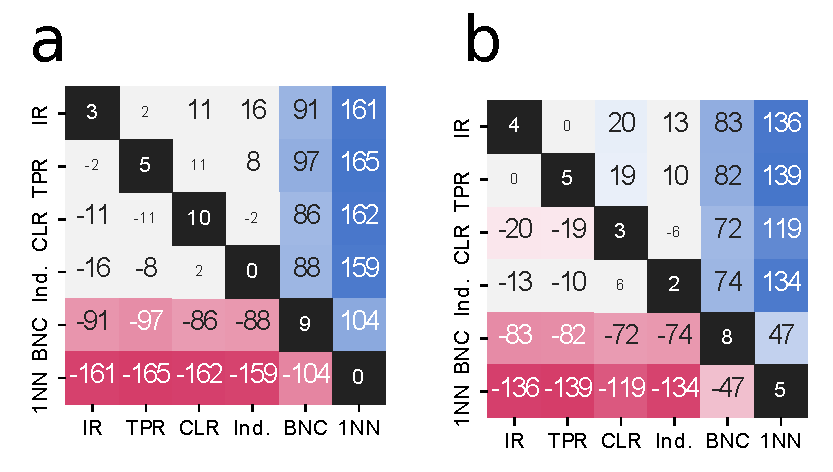
\includegraphics[width=13cm]{figures/bulk_test_pairwise_heatmaps.pdf}}
    \caption{\textbf{Pair-wise comparison of methods on bulk RNA-seq test set.} Heatmaps displaying the pair-wise difference in the number of cell types for which one method beats the other method by more than 0.05 for all pairs of methods using (a) per-cell-type average-precision score and (b) per-cell-type achievable recall at 0.9 precision. For each pair of methods, we also perform a Wilcoxon signed-rank test to assess the whether there exists a significant difference in (a) average precision values and (b) achievable recall at 0.9 precision across the cell types.  We note that this test will be aggressive as the average precision values across cell types are not independent. We bold the entries in the heatmap when p $<$ 0.05.  The diagonal entries present the number of cell types for which the corresponding row's method beat all other methods in (a) average-precision and (b) achievable recall at 0.9 precision by more than 0.05.}
    \label{fig:bulk_pairwise}
      \end{figure}

\subsection*{Evaluation on single-cell RNA-seq data}

We trained the IR, TPR, and CLR algorithms on the entire set of bulk RNA-seq data and evaluated them on the test set consisting of \BulkRestrictedSingleCellExperiments{} single-cell RNA-seq samples whose cell types appear in the bulk RNA-seq training data. We note that many cells were labeled as a broad cell type rather than a specific cell type. For example, in study ERP017126, many cells are described by the data as general pancreatic cells. These samples are likely missing cell type labels because they should, in theory, be labeled with a specific cell type (i.e., lower in the ontology) due to the facts that each sample originates from a single cell and that there are known subtypes of pancreatic cells.  We therefore modified our evaluation metrics to take into account these ambiguous, generally-labeled single-cell samples so as not to penalize the algorithms for predicting cell types more specific than their given labels. We found that these algorithms perform well in all modes of evaluation using these modified metrics (Fig.~\ref{fig:results_test_single}, Fig.~\ref{fig:sc_pairwise}, Fig.~\ref{fig:sc_pr_curves}). 

 \begin{figure}[h!]
       \centerline{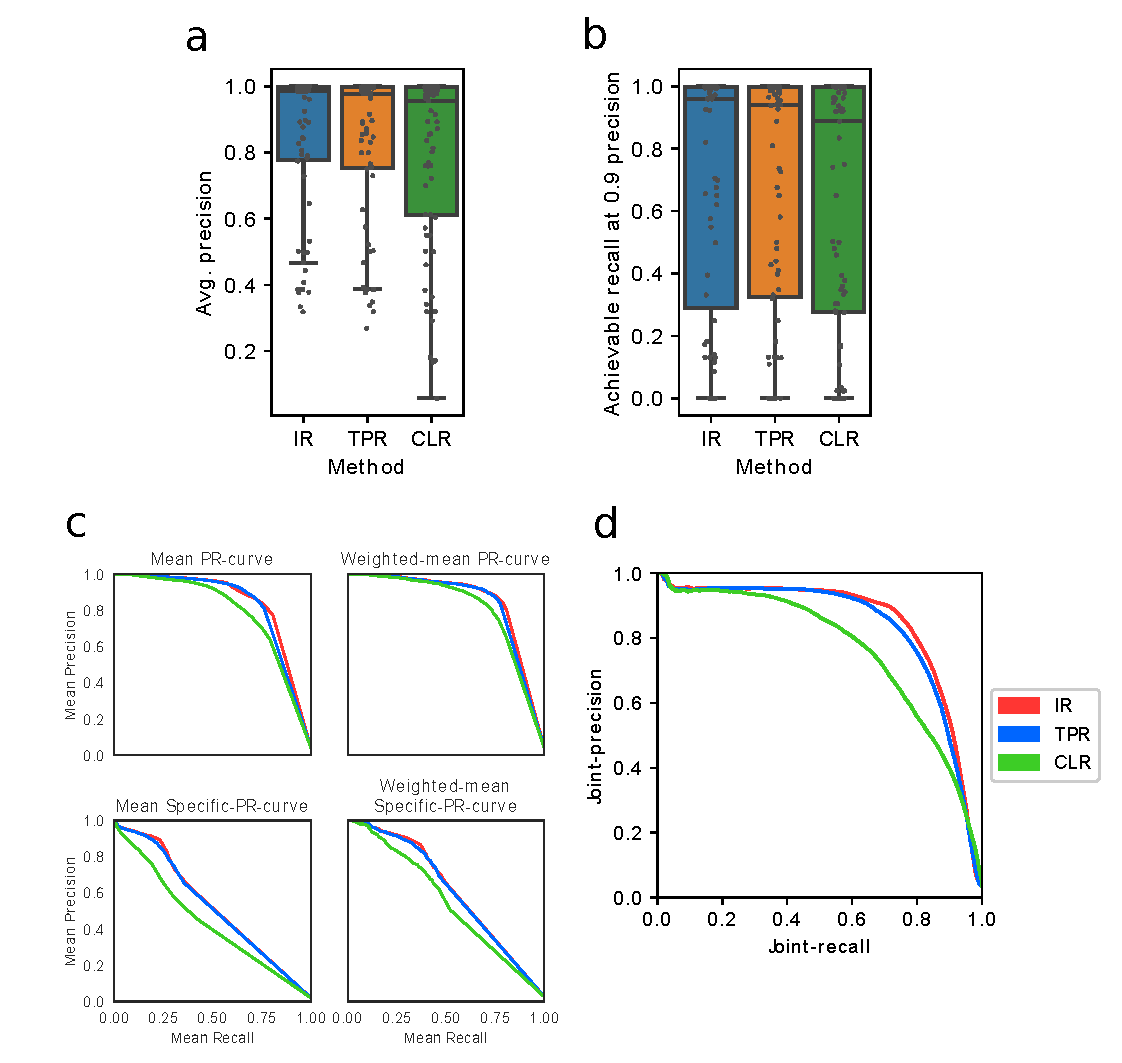
\includegraphics[width=13cm]{figures/single_cell_test_results.pdf}}
       \caption{\textbf{Single-cell test set results.}  (a) Comparison between the distributions of average-precision generated by each method across all cell types.  (b) Comparison of the distributions over the highest achievable recalls when precision is fixed at 0.9 across all cell types. (c) Variants of the mean precision-recall curves for comparing the average performance of each method across all samples. (d) The joint-precision recall curves for all methods generating by ranking all sample-cell type output probabilities jointly.}
      \label{fig:results_test_single}
      \end{figure}

\begin{figure}[htbp]
    \centerline{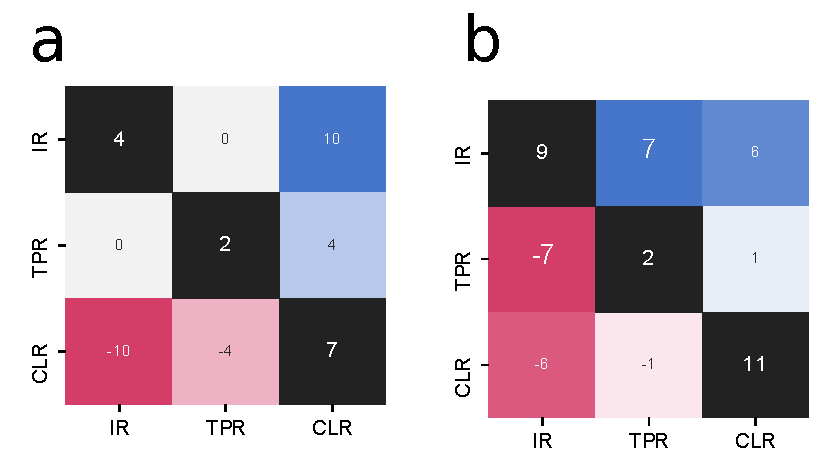
\includegraphics[width=13cm]{figures/sc_pairwise_heatmaps.pdf}}
    \caption{\textbf{Pair-wise comparison of methods on bulk RNA-seq test set.} Heatmaps displaying the pair-wise difference in the number of cell types for which one method beats the other method by more than 0.05 for all pairs of methods using (a) per-cell-type average-precision score and (b) per-cell-type achievable recall at 0.9 precision. For each pair of methods, we also perform a Wilcoxon signed-rank test to assess the whether there exists a significant difference in (a) average precision values and (b) achievable recall at 0.9 precision across the cell types.  We note that this test will be aggressive as the average precision values across cell types are not independent. We bold the entries in the heatmap when p $<$ 0.05.  The diagonal entries present the number of cell types for which the corresponding row's method beat all other methods in (a) average-precision and (b) achievable recall at 0.9 precision by more than 0.05.}
    \label{fig:sc_pairwise}
      \end{figure}

 \clearpage
\begin{sidewaysfigure}%
    \thispagestyle{empty}
    \hspace{-7cm}
    \centering
    {{\includegraphics[width=24cm]{figures/sc_pr_curves_on_graph.pdf} }}%
    \qquad
    {\hspace*{-10cm}{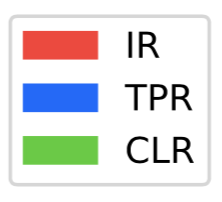
\includegraphics[width=2cm]{figures/sc_legend.png} }}%
    \caption{\textbf{scRNA-seq test set precision-recall curves.} Precision-recall curves for each cell type on the scRNA-seq test dataset. Each node is colored according to which method yielded the highest average precision. The intensity of the color corresponds to the difference between the highest average-precision and the second highest average-precision achieved for that node.}%
    \label{fig:sc_pr_curves}%
\end{sidewaysfigure}
\clearpage

Next, we examined the predictions performed on cells that represented challenging cases for the classifiers. Specifically, we identified two categories of challenging samples: samples that were only  labeled with a broad cell type and samples labeled with a combination of cell types that do not appear in the training data. We examined two studies, SRP067844 and ERP017126, that contained samples that were representative of these challenges and examined their predictions in depth.

When given samples labeled as a general cell type, but not a more specific cell type, the algorithm often predicted a more specific cell type than the labeled cell types.  Study SRP067844 included a set of samples labelled only as embryonic, neural cells, but not as a more specific cell type. In such instances, the algorithm often labeled them as the more specific label, ``neuron", which may be accurate given that this study sought to sequence cells from the developing nervous system (Fig.~\ref{fig:difficult_single_cells}a) (\citealp{Manno2016}). Study ERP017126 contained a set of pancreatic cells that were unlabeled for a specific pancreatic cell type.  Many of these cells were predicted as a specific endocrine cell type such as pancreatic alpha cells (Fig.~\ref{fig:difficult_single_cells}b).

When the methods were provided a query that should be assigned with a combination of labels that it had not seen before during training, its outputs were reasonable. Study SRP067844 consisted of embryonic neural cells. Although the training data contains samples of both embryonic cells and cells of various neural cell types, it does not contain any sample labeled as \textit{both} neural cell \textit{and} embryonic cell. For these samples, we found that the algorithm was often able to label these samples as ``neural cell", but often failed to label them as ``embryonic cell". Furthermore, the algorithm had difficulty labeling these samples with their specific neural cell types such as ``radial glial cell" (Fig.~\ref{fig:difficult_single_cells}c). Similarly, study ERP017126 contained various pancreatic cell types that did not exist in the training data such as pancreatic delta cells and pancreatic ductal cells. We found that the delta cells were often predicted correctly as enteroendocrine cells (Fig.~\ref{fig:difficult_single_cells}d) and were not confused with similar pancreatic endocrine cell types such as alpha cells or beta cells. Similarly, pancreatic ductal cells were often predicted as secretory cells (Fig.~\ref{fig:difficult_single_cells}e). Although the term ``secratory cell" is not an ancestral term of ``pancreatic ductal cell" in the Cell Ontology, these predictions may nonetheless be considered correct predictions given that pancreatic ductal cells are known to secrete biocarbonate (\citealp{Grapin-Botton2005}). 
  
\clearpage
 \begin{sidewaysfigure}
    \thispagestyle{empty}
    %\vspace{-4.5cm}
    \centerline{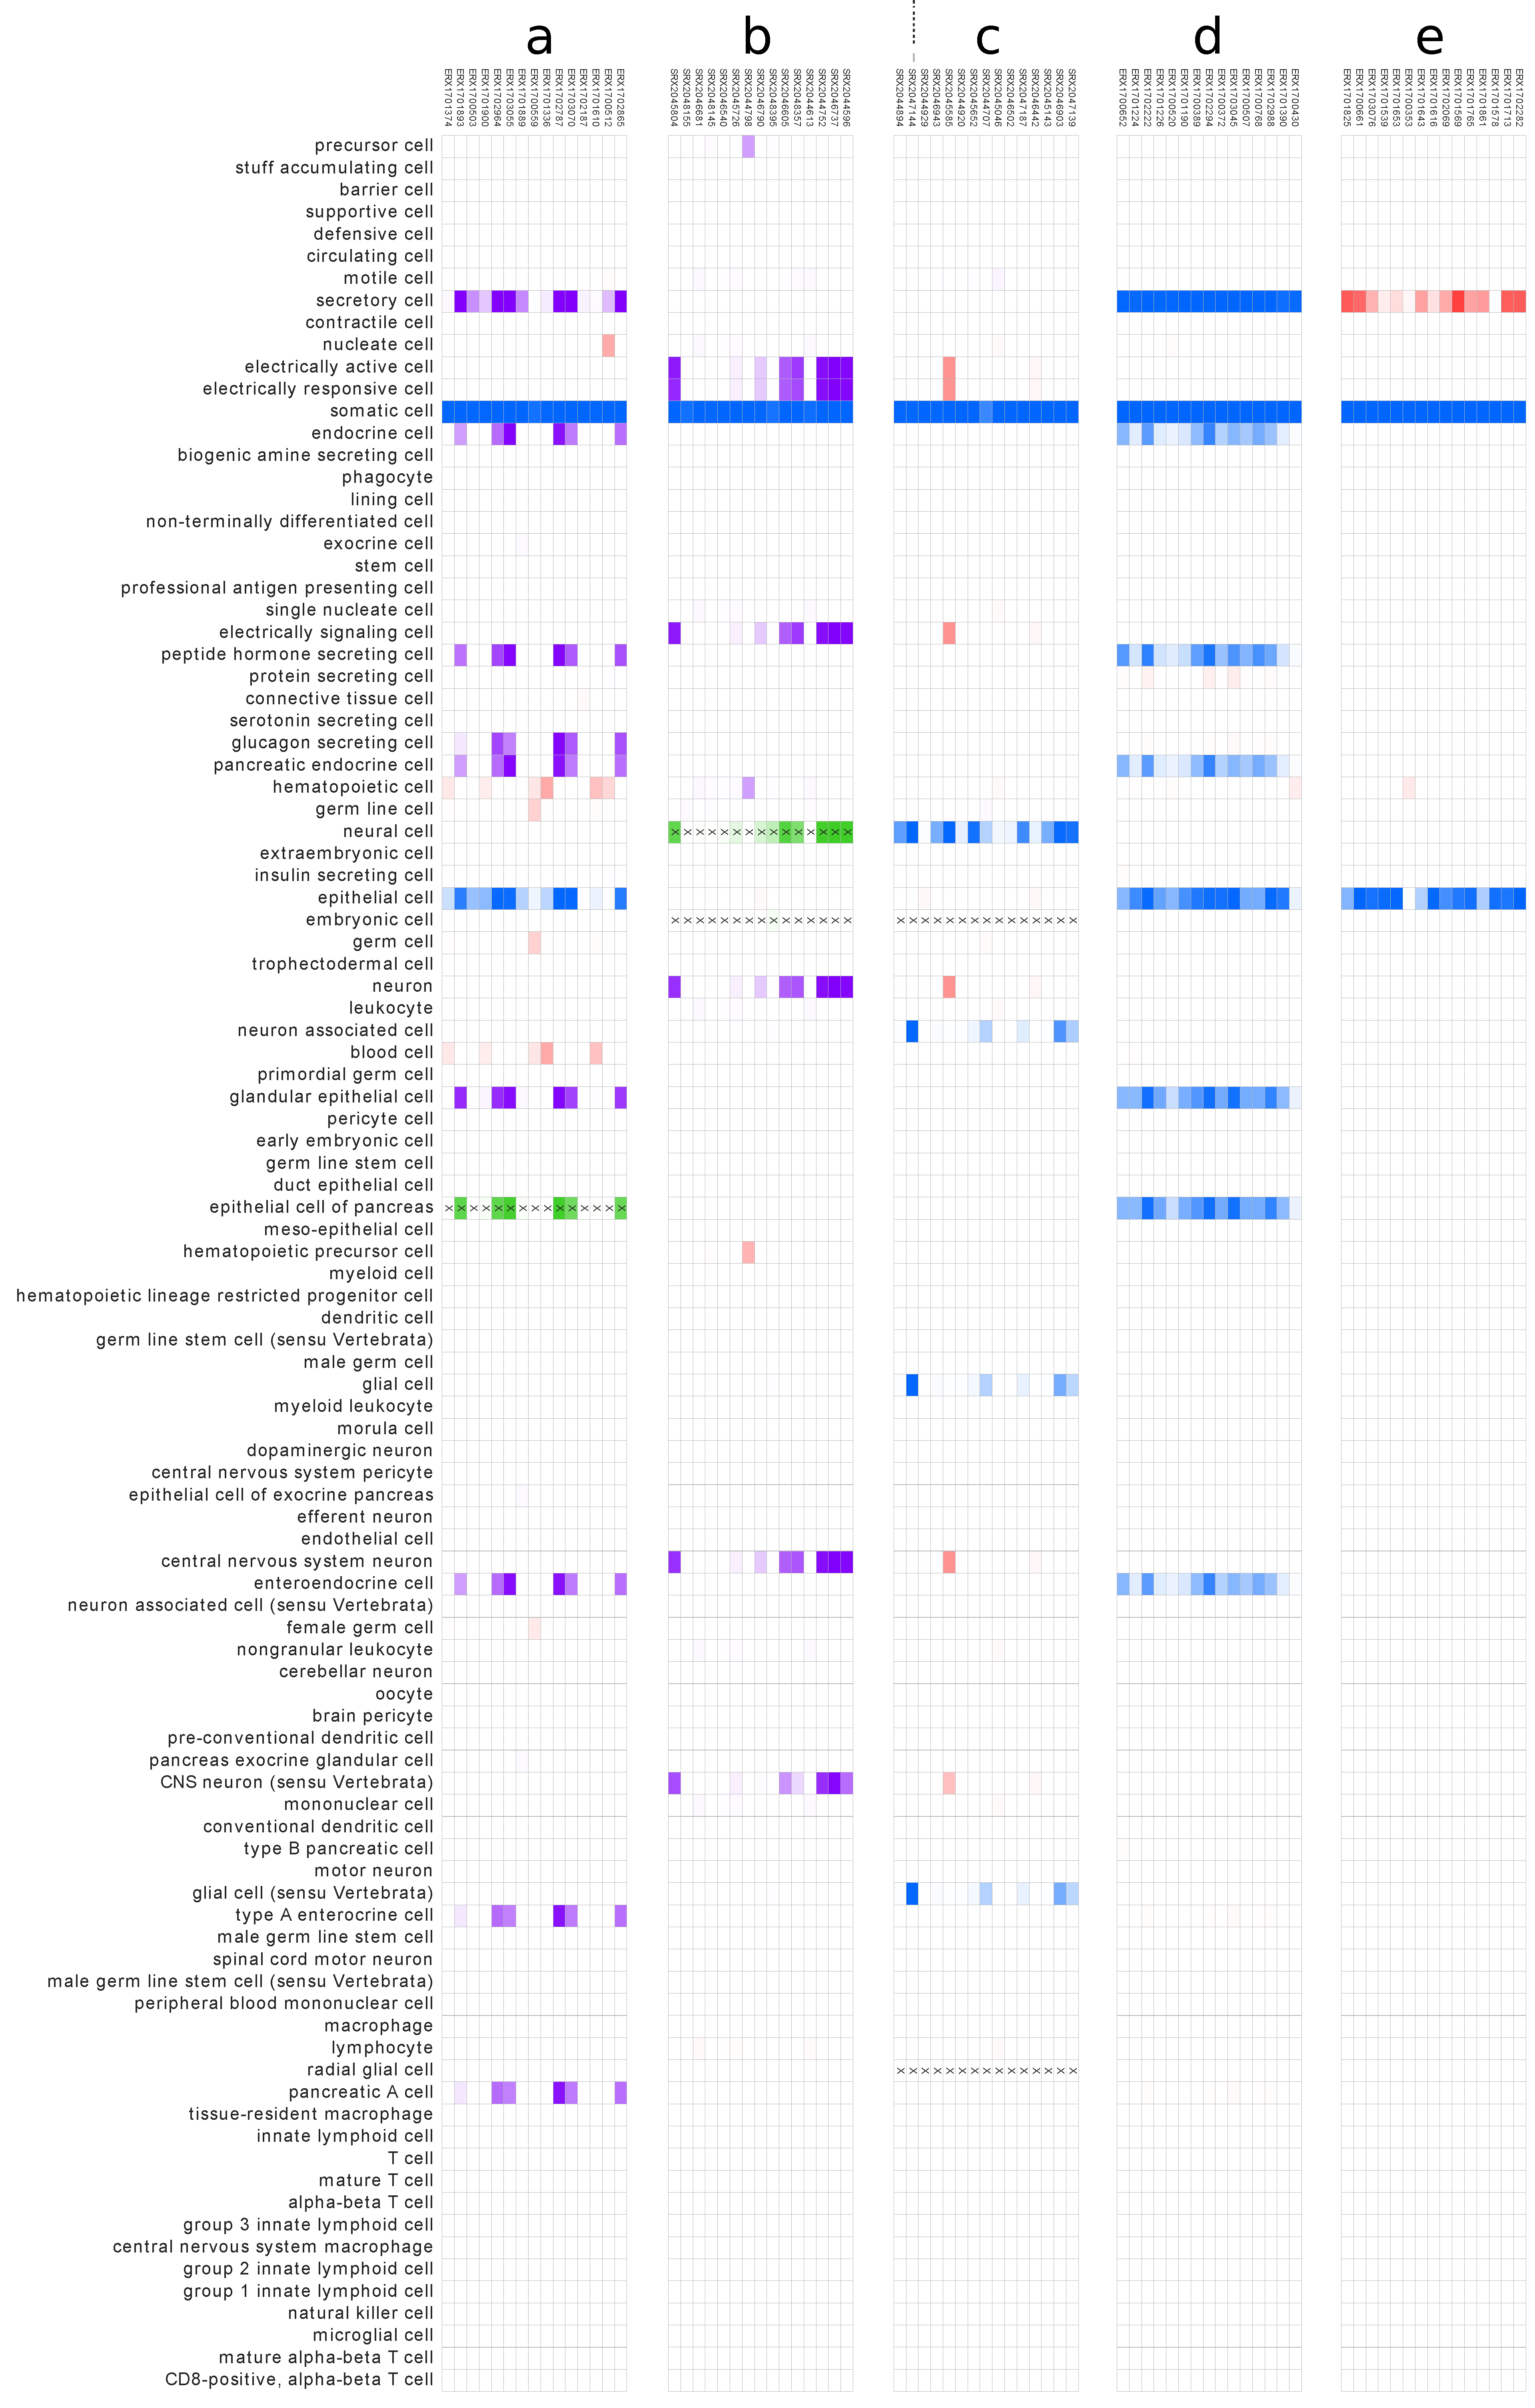
\includegraphics[scale=0.20, angle=-90]
    {figures/all_prediction_matrices_subsamples.pdf}}
   \caption{\textbf{Predictions on challenging single-cell samples.} Randomly sampled output from the IR classifier on difficult-to-classify single-cell samples. Columns correspond to cells and rows correspond to cell types that appeared in the training data. The intensity of each element is proportional to the output probability for the corresponding sample and cell type. Each element is colored according to the relationship between the sample and the cell type. Green denotes a prediction of a most-specific true cell type (annotated with an 'X') for the sample. Blue denotes a prediction of a less-specific, but true cell type. Purple denotes ambiguous predictions that cannot be verified as correct or incorrect (descendents of the sample's true cell types as well as ancestors of those descendents). Red denotes a likely error (a cell type that is neither a true cell type, descendant of a true cell type, nor ancestor of a descendent of a true cell type). We investigated the predictions of samples that are labeled as general cell types, but not more specific cell types from studies ERP017126 (a) and SRP067844 (b). We also investigated predictions on cell types that did not appear in the training data including embryonic radial glial cells (c), delta cells (d), and ductal cells (e).}
    \label{fig:difficult_single_cells}
      \end{sidewaysfigure} 
        
  
\subsection*{Comparison of interpretability between frameworks}

With the exception of the one-nearest neighbor classifier, the methods that we have explored can be subdivided into two categories: those that train a set of one-versus-rest binary classifiers (BNC, IR, TPR) and the CLR framework, which trains a set of ``local" binary classifiers that classify a sample as a given cell type conditioned on the sample belonging to its parent cell types. We explored the question of whether one framework provides an advantage in model interpretability.  To address this question, we analyzed the gene coefficients in each binary classifier's linear model for enrichment of genes involved in known biological processes. We use the number of enriched biological processes as a quantitative measure of model interpretability.  
Specifically, for each learned binary classifier, we rank the genes by their corresponding coefficients in the linear model. We then performed a gene set enrichment analysis with GSEA (\citealp{Subramanian2005}) on these ranked genes using all  ``biological process" gene sets from the Gene Ontology (GO) (\citealp{Ashburner2000}) that were associated with at least \MinGenesInGOSet{} genes. This analysis targeted enrichment at both the top and bottom of the ranked list of genes, which identified biological processes that were either relatively upregulated or downregulated in a given cell type. We then use a false discovery rate q-value cutoff of 0.05 for proclaiming enrichment.  

We found that the models learned in the CLR framework tended to be enriched for more GO terms than the one-versus-rest frameworks (Fig.~\ref{fig:compare_go_enrichment}). We posit that this phenomenon is due to the fact that since the CLR framework involves the training of binary classifiers that seek to distinguish only between a small set of similar cell types, the CLR's classifiers are ``more focused" than the one-versus-rest classifiers, which seek to distinguish each cell type from \textit{all} other cell types.  Thus, the CLR framework may prove more useful for exploring cell type-specific expression patterns and for finding expression patterns that distinguish similar cell types.  The trained model coefficients can be downloaded for further analysis from \DataDownloadURL{}.

 \begin{figure}[h!]
    \centerline{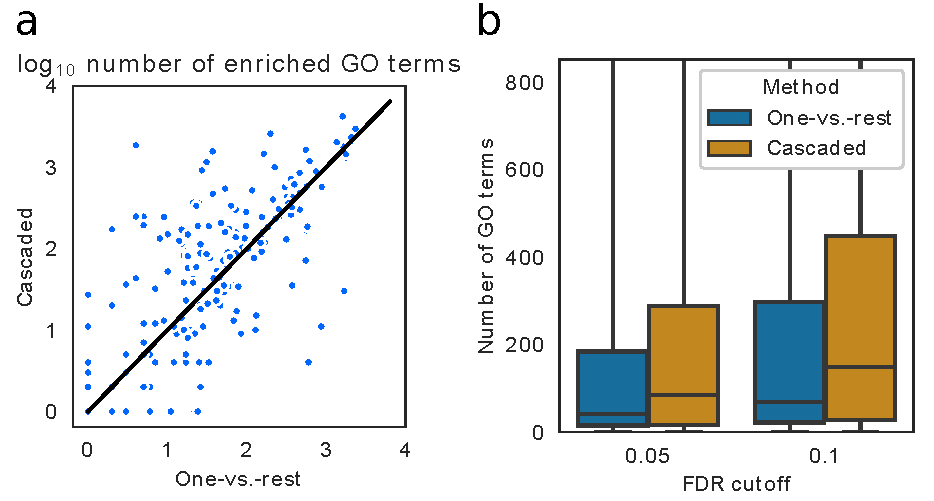
\includegraphics[width=13cm]{figures/GO_enrichment_figure}}
    \caption{\textbf{Gene set enrichment analysis on model parameters.} (a) Comparing the number of GO terms enriched in the ranked list of each binary classifier's coefficients between the cascaded logistic regression and one-vs.-rest frameworks. (b) The distribution of the number of enriched GO terms between these two frameworks using two FDR thresholds for enrichment.}
    \label{fig:compare_go_enrichment}
      \end{figure}



\section{Conclusions}

In this work, we explore the application of hierarchical classification algorithms towards cell type prediction using a novel, well-curated set of human primary cell RNA-seq samples. This dataset may prove useful for future investigations of cell type expression patterns or for use in cell type deconvolution methods (\citealp{Aran2017, Newman2015}). We demonstrate that the trained classifiers perform well across cell types on bulk RNA-seq data and offer a promising approach to cell type annotation in single cell datasets.  

We also found that classification performance is not only dependent on the number of training samples, but also on the diversity of those samples. Specifically, we found that the classifier benefits from training on data from multiple studies. Thus, we argue that the heterogeneity present in the public expression data presents an opportunity to learn robust models. This observation may extend beyond cell type prediction to other phenotype prediction tasks such as expression-based disease prediction.

Furthermore, by using linear models, the trained parameters are easily interpreted as cell type specific signatures across the ontology.  However, we note that since certain cell types undergo similar sorting and preparation procedures (e.g., fluorescence activated cell sorting), it remains unclear to what extent these procedures affect gene expression and thus confound with cell type. We sought to mitigate this effect by using data from a diversity of studies.  We also note that the CLR algorithm may help to further mitigate this effect, since the binary classifiers trained in this framework for each cell type condition on the sample belonging to the parent cell types. Thus, for a given cell type, if the parent cell types were prepared through similar procedures, the learned model parameters for that cell type will better capture biological cell type signatures. 

Finally, we expect the performance of hierarchical classifiers to improve as both more data is collected and as the Cell Ontology is expanded. More data will be collected both as data is continually added to the SRA and as improvements are made to the SRA's metadata thereby allowing retrieval of previously undiscovered primary cell samples.   

\section{Methods}
A schematic diagram of the experiments performed in this chapter is given in Figure~\ref{fig:cell_type_setup}.

\begin{figure}[htbp]
    \centerline{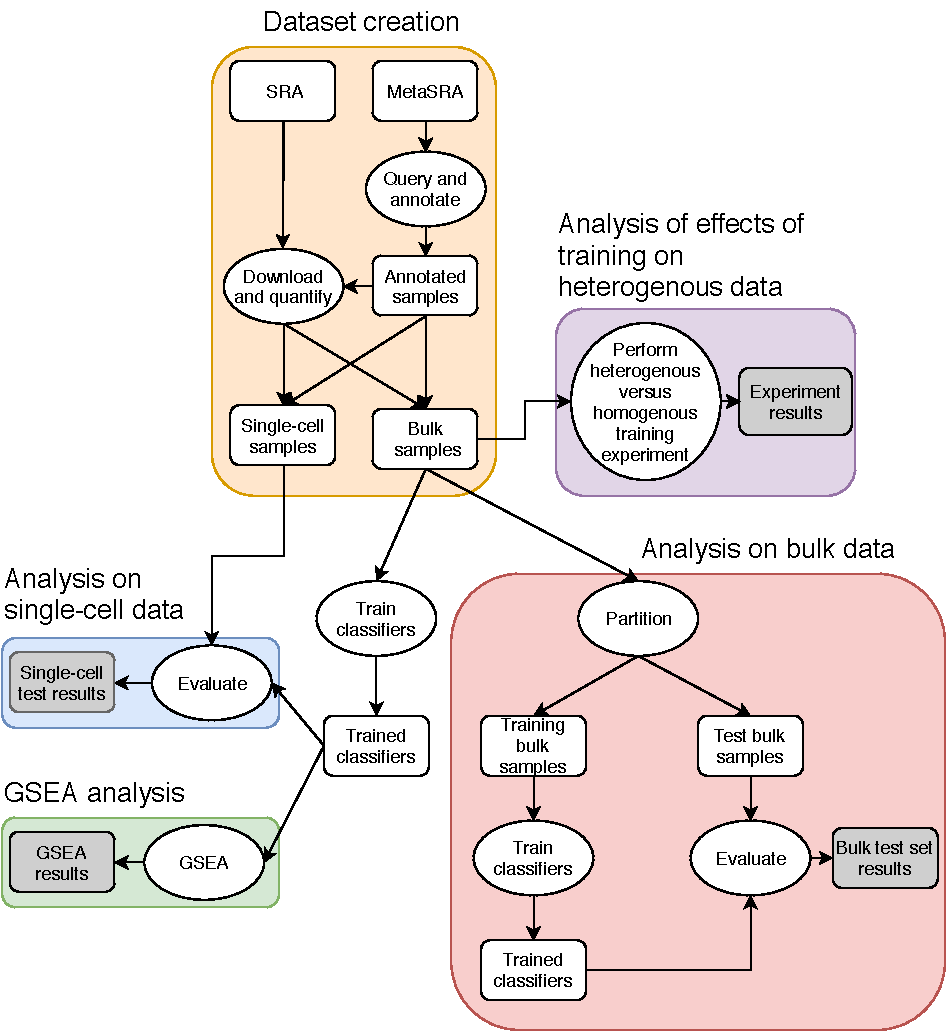
\includegraphics[width=13cm]{figures/cell_type_prediction_setup.pdf}}
    \caption{\textbf{Data flow diagram.} A data flow diagram illustrating data retrieval, annotation, partitioning, training, and analysis involved in this work.}
    \label{fig:cell_type_setup}
      \end{figure}

\subsection*{Data processing}

We quantified the gene expression of all samples with kallisto (v0.43.1) (\citealp{Bray2016}) against the human genome release GRCh38 with GENCODE annotation version 27. We chose kallisto for gene expression quantification in order to prioritize processing speed on this large dataset, figuring that any small loss in accuracy (at the gene level) relative to a less approximate, but slower method would not be significant for the cell type classification task. This produced estimated counts for \RawGenomicFeatures{} isoform-level genomic features. We summed these counts by gene to produce counts for \GeneLevelFeatures{} gene-level features. The curated metadata and associated quantified samples are available to download at \DataDownloadURL{}.


\subsection*{Partitioning bulk RNA-seq data into training and test sets}

When creating a training and test partition of the bulk RNA-seq data, we sought to satisfy a number of criteria that would enable unbiased estimation of performance across cell types:

\begin{enumerate}
    \item No study should be split between the training and test sets. This mitigates the possibility that the algorithm will provide an overly optimistic estimate of the generalization error when run on the test set. 
    \item 80/20 split of the data between the training and test sets.
    \item Maximized overlap of cell types in both the training and test sets to enable training and evaluation on as many cell types as possible.
    \item  For all cell types represented by three or more studies, at least two of those studies should be assigned to the training set. This criteria enables us to perform leave-study-out cross-validation only on the training set, thereby allowing us to evaluate various algorithms on the training set before performing a final analysis on the test set.  
\end{enumerate}
We formulate the data partitioning problem as an optimization problem and attempt to arrive at a ``best" partition that balances the aforementioned four goals.

For this section, we will use the following notation: Let $\mathcal{C}$ be the set of cell types represented in our data. Let $m$ denote the number of studies representing samples in the dataset. Let $S_1, \dots, S_m$ be the sets of cell types in each study.   That is, $S_i \subseteq \mathcal{C}$ where $c \in S_i$ if a sample labeled with cell type $c$ is included in study $i$.  Since we must ensure that the training-test partition is split along study boundaries, we define indicator variables $x_1, \dots, x_m$ that indicates whether each study $i \in [m]$ is included in the training set. Let $\boldsymbol{x} \in \{0, 1\}^m$ be the vector consisting of these indicator variables. 

Using this notation, we can mathematically describe each of the aforementioned goals:
\begin{enumerate}
\item We seek a partition such that some proportion $t$ of studies are in the training set and $1-t$ are in the test set.  We set $t := 0.8$.  We can encode how far we are from achieving this goal using the following function:
$$g_1(\boldsymbol{x}) := \left| \frac{1}{m}||\boldsymbol{x}||_1 - t \right|$$
 \item We seek to maximize the number of cell types represented in both the training and test sets. We encode this goal using the following function: $$g_2(\boldsymbol{x}) := \frac{1}{\mathcal{C}}
\left|\bigcup_{i : x_i = 1} S_i \ \Delta \ \bigcup_{i : x_i = 0} S_i\right|$$
where $\Delta$ is the symmetric difference operation.  
\item For each of those cell types that are represented by at least three studies, we would like to include at least two of those studies in the training set. For a given $\boldsymbol{x}$, let $h(\boldsymbol{x})$ be the fraction of cell types represented by at least three studies that appear at least twice in the training data. Then, our third goal can be described as:
$$g_3(\boldsymbol{x}) := 1 - h(\boldsymbol{x})$$
\end{enumerate}
We then attempt to minimize the following objective function:
$$f(\boldsymbol{x}) := \lambda_1 g_1(\boldsymbol{x})  + \lambda_2 g_2(\boldsymbol{x}) + \lambda_3\ g_3(\boldsymbol{x})$$
Each term in the objective function reflects one of our goals.  The weights $\lambda_1$, $\lambda_2$, $\lambda_3$ set the importance that we place on meeting each goal.  We used a simple hill-climbing procedure to find a partition of the data that minimizes this objective function.

\subsection*{Description of algorithms}

In the following descriptions of the algorithms used in this work, we let $\boldsymbol{x} \in \mathbb{R}^G$ denote a gene expression profile, in units of log-counts per million (log-CPM), where $G$ is the number of considered genes.  Specifically, for gene $i$ in $\boldsymbol{x}$, log-CPM is defined as
$$x_i := \log\left(\left[\frac{c_i}{\sum_{j=1}^G c_j} \times 10^6\right] + 1\right)$$ where $c_i$ is the expected number of reads mapped to the $i$th gene.  We let $n$ denote the number of samples, $m$ denote the number of considered cell types, $y_i \in \{0, 1\}$ denote the cell type assignment for cell type $i \in [m]$, and $\boldsymbol{X}$ denote the training set.

\subsubsection*{Independent binary classifiers}

We used logistic regression with L2-regularization, using scikit-learn (v.0.20.2), for all independent binary classifiers trained in the CLR, IR, and TPR frameworks as well as in the independent classifier baseline method. Our choice of L2 penalty over L1 penalty was motivated by our goal of training interpretable models. Specifically, because the L1 penalty induces sparsity, we were concerned that it would lead to zeroing-out the coefficients of important cell-type-specific genes when such genes correlated highly with other predictive genes. That is, we sought for our models to weight \textit{all} genes according to their predictive ability. 


\subsubsection*{One-nearest neighbor}

Given a query gene expression profile $\boldsymbol{x}$, we return all cell type labels belonging to the training set expression profile
$$\text{arg min}_{\boldsymbol{x}' \in \boldsymbol{X}} \ 1 - \text{Corr}(\boldsymbol{x}, \boldsymbol{x}')$$
where $\text{Corr}(\boldsymbol{x},\boldsymbol{x}')$ is the Pearson correlation of the expression values in $\boldsymbol{x}$ and $\boldsymbol{x}'$.

\subsubsection*{Cascaded logistic regression}

Classification is made in a top-down fashion starting from the root of the ontology downward as proposed by Obozinski \textit{et al.} (2008). This is accomplished by training a logistic regression, binary classifier for each cell type $i \in [m]$ to model the distribution 
$$q_i := p(y_i = 1 \mid \pi_i=1, \boldsymbol{x})$$ 
where $\pi_i \in \{0, 1\}$ indicates whether the sample belongs to all of the parents of $i$ in the ontology. In order to model these distributions, each cell type's negative training examples consist of those samples that are labeled with all parent cell types, but not the target cell type. Given these learned distributions, the probability that $\boldsymbol{x}$ originates from cell type $i$ is computed via  
$$p(y_i = 1 \mid \boldsymbol{x}) = q_i \prod_{j \in A_i} q_j$$ 
where $A_i$ denotes the ancestors of cell type $i$ in the ontology's DAG. 

\subsubsection*{Bayesian Network Correction}

A support vector machine (SVM) binary classifier is trained for each cell type using a linear kernel and a one-versus-rest training strategy. The classifier outputs are then reconciled with the ontology graph using a Bayesian network as proposed by Lee \textit{et al.} (2013).  The true assignments for each cell type, denoted $y_1, \dots, y_m$, are modelled as latent random variables, and the classifier outputs, denoted $f_1(\boldsymbol{x}), \dots, f_m(\boldsymbol{x})$ (signed distances to each decision boundary), are modelled as observed random variables in a Bayesian network.  The final output probability for cell type $i$ is then the marginal probability
$$p(y_i = 1 \mid f_1(\boldsymbol{x}), \dots, f_m(\boldsymbol{x}))$$
Due to the size of the ontology, we perform approximate inference using Gibbs sampling rather than exact inference using the Laurintzen algorithm as was performed by Lee \textit{et al.}.

\begin{figure}[htbp]
    \centerline{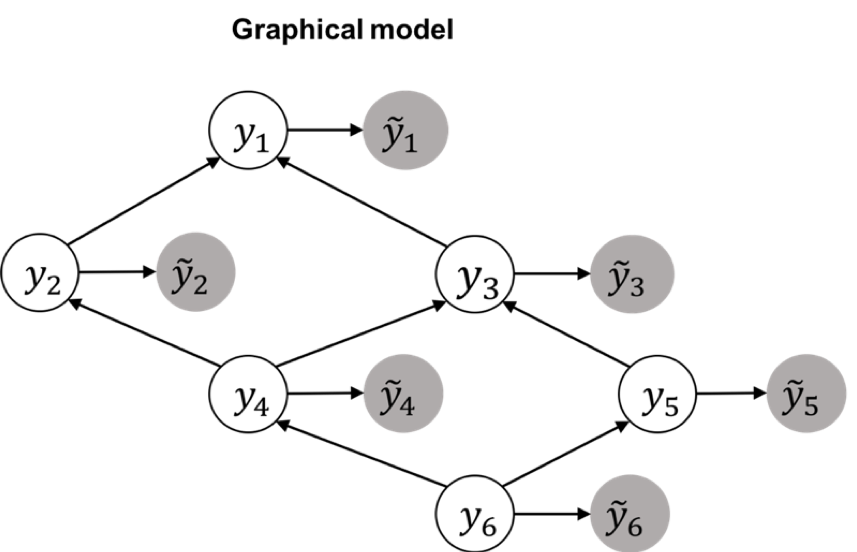
\includegraphics[width=8cm]{figures/BNC_graph.png}}
    \caption{\textbf{Bayesian Network Correction.} An example Bayesian network used in the BNC approach.  Here, $\tilde{y}_i := f_i(\bold{x})$ is the random variable representing the SVM score (i.e. signed distance of the hyperplane) of a feature vector $\bold{x}$ according to the trained SVM classifier for cell type $i$.}
    \label{fig:cell_type_setup}
      \end{figure}

\subsubsection*{Isotonic regression correction}

We train a binary classifier for each cell type $i \in [m]$ to model $p(y_i \mid \boldsymbol{x})$ using logistic regression and a one-versus-rest training strategy.  As proposed by Obozinski \textit{et al.} (2008), these probabilities are then reconciled with the ontology graph using isotonic regression. Specifically, we output the set of probabilities 
$$p_1, \dots, p_m := \text{arg min}_{p'_1, \dots, p'_m} \sum_{i=1}^m (p'_i - \hat{p_i})^2$$
subject to 
$$\forall i \in [m], \forall j \in \text{Par}(i), \ p_i < p_j$$
where $\forall i \in [m], \hat{p}_i := p(y_i=1 \mid \boldsymbol{x})$ as output by each classifier and $\text{Par}(i)$ is the set of parent cell types for cell type $i$. 

\subsubsection*{True Path Rule}

We train a binary classifier for each cell type $i \in [m]$ to model $p(y_i \mid \boldsymbol{x})$ using logistic regression and a one-versus-rest training strategy.  As proposed by Notaro \textit{et al.} (2017), this method involves two passes across the ontology: on a bottom-up pass, each cell type's output probability is averaged with the outputs of all child cell types classifiers for which the classifier makes a positive prediction according to a predefined threshold.  More specifically, each cell type $i$'s output probability is set to
$$p_i := \frac{1}{|C_i|+1}\left(\hat{p}_i + \sum_{j \in C_i} \hat{p}_j\right)$$
where $\hat{p}_i := p(y_i=1 \mid \boldsymbol{x})$ according to the classifier and 
$$C_i := \{j \in \text{Children}(i) \ : \ \hat{p}_i > t \}$$ 
is the set of children of cell type $i$ for which the classifier output a positive prediction according to a predefined threshold $t$. We used a threshold of $t = 0.5$.  This bottom-up pass allows sharing of information across the classifiers. In the top-down pass of the ontology, the output probabilities are set to ensure consistency with the ontology.

\subsection*{Per-sample evaluation metrics}

In the per-sample mode of evaluation, we analyze the average performance over each sample. For a given sample, let $T$ be the full set of a true cell type labels and $P$ be the set of predicted labels. The per-sample precision and recall are then defined as
$$
   \text{Precision} := \left\{
     \begin{array}{lr}
       \frac{|T \cap P|}{|P|} & : |P| > 0  \\
       1 & : |P| = 0
     \end{array}
   \right.
$$
$$\text{Recall} := \left\{
     \begin{array}{lr}
       \frac{|T \cap P|}{|T|} & : |T| > 0  \\
       1 & : |T| = 0
     \end{array}
   \right.$$
respectively.  We further define a version of precision and recall, termed \textit{specific-precision} and \textit{specific-recall}, that seek to summarize how well the classifier is retrieving the most granular cell types that describe the sample. Given a cell type label $c$ from the ontology, let $Ch(c)$ be the children of $c$ in the ontology DAG. We then define the most-specific set of true labels and most-specific set of predicted labels as
$$T' := \{c \in T : |Ch(c) \cap T| = 0 \}$$
$$P' := \{c \in P : |Ch(c) \cap P| = 0 \}$$
respectively. Specific precision and recall are then defined as
$$\text{Specific-Precision} := \left\{
     \begin{array}{lr}
       \frac{|T \cap P'|}{|P'|} & : |P'| > 0  \\
       1 & : |P'| = 0
     \end{array}
     \right.$$
$$\text{Specific-Recall} := \left\{
     \begin{array}{lr}
       \frac{|T' \cap P|}{|T'|} & : |T'| > 0  \\
       1 & : |T'| = 0
     \end{array}
     \right.$$
respectively. Given these per-sample measures of precision and recall, we then compute mean precision (MP), mean recall (MR), mean specific-precision (MSP), and mean specific recall (MSR) across all samples. 

Finally, as was noted previously, since samples from the same study perform similarly, these metrics will be most effected by these large studies. To counteract this effect we also define a set of average metrics that use a weighted mean so that each study contributes equally. These metrics, which we call weighted-mean precision (WMP), weighted-mean recall (WMR), weighted-mean specific-precision (WMSP), and weighted-mean specific-recall (WMSR) are defined as
$$WMP := \frac{1}{s}\sum_{i=1}^n \frac{1}{|S_i|}\text{Precision}_i$$
$$WMR := \frac{1}{s}\sum_{i=1}^n \frac{1}{|S_i|}\text{Recall}_i$$
$$WMSP := \frac{1}{s}\sum_{i=1}^n \frac{1}{|S_i|}\text{Specific-Precision}_i$$
$$WMSR := \frac{1}{s}\sum_{i=1}^n \frac{1}{|S_i|}\text{Specific-Recall}_i$$
where $n$ is the total number of samples, $s$ is the total number of studies, and $S_i$ is the set of samples in the study that includes sample $i$. Finally, by varying the prediction threshold, we can compute curves for all of these metrics. Specifically, we compute mean PR-curves, mean specific-PR-curves, weighted-mean PR-curves, and weighted-mean specific-PR-curves.

\subsection{Modified single-cell evaluation metrics}

When evaluating performance of the classifiers on the single-cell test dataset, we modified the evaluation metrics to take into account samples that were labelled with a general cell type, but not a specific cell type. The ground-truth for these more-specific cell types are ambiguous since these samples should, in theory, be labelled with a specific cell type (i.e., a cell type that is low in the ontology DAG) due to the fact that they originate from single cells.  This stands in contrast to bulk RNA-seq samples that may constitute a population of specific cell types for which it would be apt to label such samples with the less specific cell type that covers all of the cell types in the population (e.g. labelling a bulk RNA-seq sample as ``T cell" when it constitutes a heterogeneous population of T cell subtypes).  For many of these ambiguous single-cell samples, we found that the classifier would output a high probability for a more specific cell type than that with which it was labelled. Such predictions by the classifier cannot be verified and therefore we argue that they should neither be rewarded nor penalized in our evaluation metrics. Therefore we modified as metrics as described in the sections below.

\subsubsection{Per-cell type mode of evaluation}

When constructing the precision-recall curves for a given cell type, we exclude those samples that are labelled most-specifically as an ancestor of the cell type. For example, we would exclude from the ``CD8-positive alpha-beta T cell" precision-recall curve those samples that are most-specifically labelled as ``T cell". 

\subsubsection{Per-sample mode of evaluation}

To modify the specific-precision and specific-recall metrics, we take into account those cell types that are more specific than the true cell type label and those cell types that are ancestors of these more-specific labels. For a given sample, let $T$ be the set of true cell type labels and let $P$ be the set of predicted cell type labels. Furthermore, we the define the most specific true cell type labels and most specific predicted labels as 
$$T' := \{x \in T : |Ch(x) \cap T| = 0 \}$$
$$P' := \{x \in P : |Ch(x) \cap P| = 0 \}$$
respectively where $Ch(x)$ is the set of children of cell type $x$ in the ontology.  For a given cell type $x$, let $A(x)$ be the ancestors of $x$ and let $D(x)$ be the descendents of $x$. Then, let $M$ be the descendents of the most specific true cell types. That is,
$$M := \bigcup_{x \in T'} D(x)$$
Since the ontology is a DAG, it holds that $M \cap T = \emptyset$.
We can now define all of the ambiguous cell types as
$$R := M \cup \left(\bigcup_{x \in M} (A(x) \setminus T)\right)$$
Now, we can modify the most-specific predicted labels to be the set of most-specific predicted labels \textit{only} among those cell types that were predicted \textit{and} that are not ambiguous. That is, we define the modified most-specific predicted labels to be
$$P^* := \{x \in (P \setminus R) : |Ch(x) \cap (P \setminus R)| = 0 \}$$
Per-sample precision and recall are then modified to be defined as
$$\text{Precision} := \left\{
     \begin{array}{lr}
       \frac{|T \cap (P \setminus R)|}{|P \setminus R|} & : |P \setminus R| > 0  \\
       1 & : |P^*| = 0
     \end{array}
     \right.$$
$$\text{Recall} := \left\{
     \begin{array}{lr}
       \frac{|T \cap (P \setminus R)|}{|T|} & : |T| > 0  \\
       1 & : |T| = 0
     \end{array}
     \right.$$
respectively.  Specific-precision and specific-recall are then modified to be defined as
$$\text{Specific-Precision} := \left\{
     \begin{array}{lr}
       \frac{|T \cap P^*|}{|P^*|} & : |P^*| > 0  \\
       1 & : |P^*| = 0
     \end{array}
     \right.$$
$$\text{Specific-Recall} := \left\{
     \begin{array}{lr}
       \frac{|T' \cap (P \setminus R)|}{|T'|} & : |T'| > 0  \\
       1 & : |T'| = 0
     \end{array}
     \right.$$
respectively. 




      
         
 

      
       
       
     



% Sentence fragments

% This stands in contrast to bulk RNA-seq data for which it may be suitable to label the samples with less specific cell types when the samples consist of heterogeneous cell types. 

%Over the course of this project, we flagged a number of errors in the Cell Ontology and reported these issues to the Cell Ontology curators.  
